\section{ Preliminaries and Notation}
At the beginning of this chapter we repeat the basic definitions and notation for the analysis of partial differential equations as they are introduced for example in \cite[Introduction]{Evans1998}.
Let $\Omega \subset \R^d $ be an open, bounded area and $\partial \Omega$ its boundary.
\begin{definition}[Partial Differential Equation{\cite[Introduction]{Evans1998}}]
 A \emph{partial differential equation} (PDE) of order $k\in \N$ is an expression of the form
\begin{align}
	F(D^k u(x), D^{k-1}u(x), \dots, Du(x), u(x), x) = 0, (x \in \Omega)\label{eq:general PDE}
\end{align}
where $F:\R^{n^k} \times \R^{n^{k-1}} \times \dots \times \R^n \times \R \times \Omega \rightarrow \R $ is given and $u:\Omega \rightarrow \R$ is unknown.
\end{definition}
We focus in this thesis on second-order PDEs for our main PDE, namely the \emph{\MA equation} which we will introduce later is of second order. 
\\Next to the order there exist further properties to categorise PDEs:
\begin{definition}[Categories of PDEs{\cite[Introduction]{Evans1998}}]
	Given functions  $f:\Omega \rightarrow \R$ and $a_{\alpha}:\Omega \rightarrow \R$ or $a_{\alpha}:\R^{n^{k-1}} \times \dots \times \R^n \times \R \times \Omega$ respectively, for $\alpha \in \N^{k}, |\alpha| \leq k$, a PDE of order $k$ is called
	\begin{enumerate}[(i)]
		\item \emph{linear} if it can be written in the form
		\[
			\sum_{|\alpha| \leq k} a_{\alpha} (x) D^{\alpha} u(x) = f(x).
		\] 
		
%		\item \emph{semilinear} if it can be written in the form
%		\[
%			\sum_{|\alpha| = k} a_{\alpha}(x) D^{\alpha} u + a_0(D^{k-1}u, \dots, Du, u, x)= f(x),
%		\]	
%		i.e. a semilinear PDE is nonlinear in the unknown function, but linear in all partial derivatives.
		
		\item \emph{quasilinear} if it can be written in the form
		\[
			\sum_{|\alpha| = k} a_{\alpha}(D^{k-1}u, \dots, Du, u, x) D^{\alpha} u + a_0(D^{k-1}u, Du, u, x)= f(x),
		\]	
		i.e. a quasilinear PDE is nonlinear in (at least) on lower derivate, but linear in the highest order derivates.
		
		\item \emph{fully nonlinear} if it depends nonlinearly upon the highest order derivatives.
	\end{enumerate}
\end{definition}
A famous example for linear PDEs is the \emph{Poisson equation} $-\triangle u = f$,
% a semilinear PDE is for example the \emph{nonlinear Poisson equation} $-\triangle u = f(u)$.
a well-known example for quasilinear PDEs are equations of the type $\nabla \cdot (A(u) \nabla u) = f$, where $A: \R^d \rightarrow \R^{d \times d}  $. The \MA equation $\mydet {D^2 u} = f$ is part of the last category, the nonlinear PDEs. 

Another important property to classify second-order PDEs is ellipticity. 
\begin{definition}[Elliptic PDE{, \cite[p.207]{FGN2013}}]
	A fully nonlinear second order PDE is called \emph{elliptic} if its operator satisfy
	\begin{align}
		F(A,p,z,x) \leq F(B,p,z,x) \label{eq: ellipitic PDE}
	\end{align}
for all $x \in \Omega, z \in \R, p \in \R^d$ and $A,B \in \R^{d \times d}_{sym}$  with $A-B$ positive definite.

This notion is a natural extension of the ellipticity concept for first order PDEs. Interpreting a first order PDE operator as a Function depending on $D^2u, Du, u, x$, \eqref{eq: ellipitic PDE} characterises an elliptic PDE.
\end{definition}

Searching for a function $u:\Omega \rightarrow \R$ with 
\begin{align}
u=g \text{ on } \partial \Omega \label{eq: boundary}
\end{align}
for some $g:\partial \Omega \rightarrow \R$ is called a \emph{Dirichlet-boundary problem}. The function $u:\Omega \rightarrow \R$ fulfilling \eqref{eq:general PDE} and \eqref{eq: boundary} is called a classical solution of the problem. 

There are problems such that no such solution exists. A PDE of order $k$ requires its classical solution to be at least $k$ times differentiable, which is a very strong demand. To admit less regular solutions one aims for a weaker notion of a solution. Before doing this we specify some function spaces.

%\section{Functional Spaces}
According to the literature we refer by $W^{s,p}(\Omega)$ to the H\"older space, a set consisting of all $L^p(\Omega)$ functions whose distributional derivates up to order $s$ are contained in $L^ p(\Omega)$.
\todo{Sollte ich  distributional derivates erklaeren?} The special case $p=2$ are referred to as Sobolev spaces $H^s(\Omega):=W^{s,2}(\Omega)$. An additional subscript $0$ denotes the set where all functions are zero at the boundary, i.e. $H^s_0 :=\{f \in H^s(\Omega); f(x)=0 \; \forall x \in \partial \Omega\}$

Let $T$ be a triangle in $\Omega$ and spanned by the points $v_0, v_1, v_2$. We also write 
\[
	T= \langle v_0, v_1, v_2 \rangle := \{\beta_0 v_0+ \beta_1 v_1 +\beta2 v_2; 0 \leq \beta_i \leq 1, i= 0,1,2\}.
\]
The \emph{diameter} $diam(T)$ of a triangle $T$ we define as the diameter of the smallest circle containing it.
To discretise our domain $\Omega$ we subdivide it into simplices, more precisely we divide them into triangles.
\begin{definition}[Triangulation, {\cite[Definition 5.1]{Braess2003}}]
	We call a finite partition of $\Omega$ into triangles $\{T_1, \dots, T_n\}$ a feasible \emph{triangulation} $\mathcal{T}$, such that
	\begin{enumerate}[(i)]
		\item	$\overline \Omega = \bigcup_{T \in \triang} T_i$
		\item If $T_i \cap T_j$ is a point for, it is a vertex of both $T_i$ and $T_j$
		\item If $T_i \cap T_j$ is more than one point for $i \neq j$, it is an edge of both $T_i$ and $T_j$
	\end{enumerate}
	Let $h$ denote the maximal diameter $h:= \operatorname{max}\limits_{T\in \mathcal T} diam(T)$ in the triangulation $\mathcal T$, we then also refer to $\mathcal{T}$ by $\triang$. We call a triangulation \emph{regular} if every element is congruent.
\end{definition}
Note that this definition requires $\Omega$ to be a polygonal domain. However, there are extension to domain with curved boundaries: In those triangles lying at the boundary are replaced by "triangles" which have curved sides. 

\begin{figure}[H]
\usetikzlibrary{calc}

		\begin{center}
		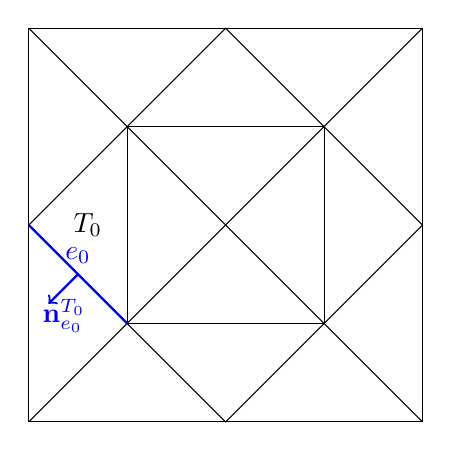
\begin{tikzpicture}[scale = 5]
%define coordinates
			\coordinate (vEins) at (0,0) ;
			\coordinate (vZwei) at (0:4cm);
			\coordinate (vDrei) at (90:4cm);

%draw square
			\draw (0,0) -- (1,0) -- (1,1) -- (0,1) -- cycle; 

%draw diagonals
			\draw (0,0) -- (1,1);
			\draw (1,0) -- (0,1);

			\draw (0.5,0) -- (1,0.5) -- (0.5,1)-- (0,0.5) --cycle; 

			\draw(0.25,0.25) -- (0.75,0.25) -- (0.75,0.75)-- (0.25,0.75) --cycle; 

			\draw node at (0.15,0.5) {$T_0$};

			\draw[color=blue, thick] (0.25,0.25)-- node[above]{\blue{$e_0$}} (0,0.5);
			\coordinate (vMiddle) ($(0.25,0.25)!0.5!(0,0.5)$);
			
			\draw[color=blue, thick, ->] ($(0.25,0.25)!0.5!(0,0.5)$) -- node[right=0.3, below=0.1]{\blue{$\mathbf n_{e_0}^{ T_0}$}} ($ ($(0.25,0.25)!0.5!(0,0.5)$) - (0.075,0.075)$);

		\end{tikzpicture}
		\end{center}

\caption{A regular triangulation of the unitsquare}
 \label{fig: triangulation}
\end{figure}

Figure \ref{fig: triangulation} shows a triangulation of the unitsquare. Since the edges uniquely define a triangulation of $\Omega$, we later use the terms grid and mesh to refer to a subdivision into triangles.
An edge $e$ is called an interior edge if $e=T^+ \cap T^-$ holds for some $T^+,T^- \in \triang$, whereas it is called a boundary edge if $e \subset \partial \Omega$.
We divide the edges $\edges$ into the subsets $\edgesi$ and $\edgesb$ containing all interior edges and boundary edges, respectively. 
When we refer to a normal of an edge we always refer to an outward directed normal of one of the adjacent triangles. If it is not clear from the context a superscript denotes which triangle we chose.

On this basis we define the piecewise spaces
\begin{definition}[Broken Spaces]
We define some function spaces associated to a triangulation
\begin{align}
	H^s(\triang) = \prod\limits_{T\in \triang}  H^s(T), \qquad W^{s,p}(\Omega) = \prod\limits_{T\in \triang} W^{s,p}(T).
\end{align}	

\end{definition}
\begin{definition}[Piecewise Polynomial Spaces] \label{def: piecewise polySpace}
	Further we denote the finite-dimensional space of piecewise polynomials by
\[	
	\mathcal P^k_h = \{ f \in L^\infty(\Omega); f \arrowvert_T \textnormal{ is a polynomial of (total) degree } \leq k \textnormal{ for every } t \in \mathcal T_h\}.
\]
\end{definition}

%\todo{norms}
We use a subscript $h$ to indicate a piecewise evaluation/interpretation. Subsequently differential operators with a subscript $h$ imply separate differentiations on every triangle.

To formulate a method capable of handling discontinuities along triangle edges we introduce edge operators.   

\begin{definition}[Edge Operators]
We denote the \emph{normal jump} of  a piecewise smooth function $u_h:\Omega \rightarrow \R$ across an edge $e \in \edges$ by
\begin{align*}
	\jump {u_h}&:= 
	\begin{cases}
		u_h^+  \mathbf n^+ + u_h^- \mathbf n^-  &\text{ if } \partial T^+ \cap \partial T^- = e \text{ for some }T^+,T^- \in \triang, \\
		u_h \mathbf n 	 &\text{ if } \partial T \cap \partial \Omega = e \text{ for } T \in \triang,
	\end{cases}	
\end{align*}
where $n^\pm$ are the normals with respect to $T^\pm$ and  $u_h^\pm(x) = \lim_{\varepsilon \rightarrow 0} u_h(x-n^\pm \varepsilon)$.
Likewise we define the normal jump of a piecewise smooth function $u_h:\Omega \rightarrow \R^2$ across an edge $e \in \edges$ by
\begin{align*}
	\jump {u_h}&:= 
	\begin{cases}
		u_h^+ \cdot \mathbf n^+ + u_h^-\cdot  \mathbf n^-  &\text{ if } \partial T^+ \cap \partial T^- = e \text{ for some }T^+,T^- \in \triang,\\
		u_h\cdot \mathbf n 	 &\text{ if } \partial T \cap \partial \Omega = e \text{ for }T\in \triang.
	\end{cases}	
\end{align*}
Here $\cdot$ denotes the scalar product.
Note, that the jump of a scalar is a vector, whereas the jump of a vector is a scalar.

The \emph{average} of a piecewise smooth function $u_h:\Omega \rightarrow X$ for every $X$ across an edge $e \in \edges$ is defined by
\begin{align*}
	\average {u_h} &:= 
	\begin{cases}
	\frac 1 2 \left(u_h^+ + u_h^-\right) &\text{ if } \partial T^+ \cap \partial T^- = e \text{ for some }T^+,T^- \in \triang, \\
	 u_h &\text{ if } \partial T \cap \partial \Omega = e \text{ for }T\in \triang.
	\end{cases}
\end{align*}
\end{definition}


\section{Finite Element Method}
Before we discuss numerical schemes for the \MA equation we shortly recall how a finite element method works, for a deeper insight in finite element methods we recommend \cite{Braess2003, BS2002}. Since the finite element method bases on a variational formulation we talk about finite element methods by the example of the general Poisson equation. 

%\subsection{The Poisson Problem}

\begin{definition}[Generalised Poisson Problem]
The \emph{Generalised Poisson Problem} is finding a function $u:\Omega \rightarrow \R$ such that 
\begin{align}
	-\nabla \cdot (A \nabla u) = f \qquad &\text{ in }\Omega \label{eq: poisson eq} \\
	u = g \qquad &\text{ on } \partial \Omega    \label{eq: poisson bc}
\end{align}
for $ A:\Omega^d \rightarrow \R^{d \times d}$ symmetric and functions $f,g:\Omega \rightarrow \R $. 
Because of the physical meaning of this PDE $A$ is also referred to as \emph{diffusion matrix}.
\end{definition}

We are able to set up a weak formulation of the Generalised Poisson Problem based on variational principles. A weak formulation of the problem is the key element for deriving a finite element method.

Due to the main theorem of variational analysis every classical solution to \eqref{eq: poisson eq} is equivalent to 
\begin{align}
	-\int_\Omega \varphi \nabla \cdot (A \nabla u) = \int_\Omega \varphi f \qquad \forall \varphi \in C^\infty(\Omega).\label{eq: variational form}
\end{align}
Integration by parts yields to
\begin{align}
	\int_\Omega \nabla \varphi  \cdot A\nabla u -\int_{\partial \Omega} \varphi (A\nabla u) \mathbf{n}  = \int_\Omega \varphi f \qquad \forall \varphi \in C^\infty(\Omega). \label{eq: FE integration by parts}
\end{align}
The last statement can be reformulated to the so called variational form 
\begin{align}
a(\varphi,u)  = b(\varphi) \qquad \forall \varphi \in C^\infty(\Omega). \label{eq: variational formulation}
\end{align}
with the bilinear form $a:C^\infty(\Omega) \times X \rightarrow \R$
\begin{align*}
a(\varphi,u) = \int_\Omega \nabla \varphi  \cdot A\nabla u -\int_{\partial \Omega} \varphi (A\nabla u) \mathbf{n}
\end{align*}
where $X$ is a function space we define in a moment and the functional $b:C^\infty(\Omega) \rightarrow \R$
\begin{align*}
 b(\varphi)  = \int_\Omega \varphi f.
\end{align*}


\begin{definition}[Weak Solution]
	Functions satisfying \eqref{eq: variational formulation} are called \emph{weak solutions} of \eqref{eq: poisson eq}.
\end{definition}
Note, due to the lack of regularity it is possible that we cannot restrict a weak solution to the boundary of $\Omega$. However one can reformulate boundary conditions for weak solution with trace operators \cite[Section 5.5]{Evans1998}.

The generalised poisson problem is well-posed in the sense that it has a unique weak solutions if $A$ is positive definite and $f\in L^2(\Omega)$. This is mainly due to the ellipticity of the PDE (and as a consequence thereof the ellipticity of $a$) allowing to apply the Lax-Milgram theory and a maximum principle. For an analysis we refer the interested reader to \cite[Chapter~6]{Evans1998}.

On the left-hand side in the weak notation only first derivatives of $u$ appear, hence \eqref{eq: variational formulation} is also applicable for functions $u$ not twice differentiable. It turned out that the previously defined Sobolev spaces are well-suited candidates for the space $X$ where we find weak solutions \cite[Chapter 1]{BS2002}. Therefore we search for the solution of the infinite-dimensional problem: Find $u\in H^1(\Omega)$ such that  $a(\varphi,u)  = b(\varphi) \;\forall \varphi \in C^\infty(\Omega)$ holds. % $\forall \varphi \in C^\infty(\Omega)$.
The main idea of the finite element method is to approximate the two function spaces, namely the spaces $H^1(\Omega)$ and $C^\infty(\Omega)$ containing $\varphi$ and $u$, respectively by finite dimensional spaces $W_h$ and $V_h$. For those spaces should hold a analogous equation as we have in the variational form stated in \eqref{eq: variational formulation}.\\
The limited space $W_h$ is called \emph{test space} and its elements are called \emph{test functions}. $V_h$ is referred to as \emph{ansatz} or \emph{trial space}, the contained functions accordingly \emph{ansatz} or \emph{trial functions}. To assert the boundary condition \eqref{eq: poisson bc} we demand $u_h|_{\partial \Omega} = g$ for every $u_h \in V_h$.

As the subscript $h$ suggests the two spaces normally are based on a discretisation of $\Omega$ and often only piecewise smooth. Consequently, since we are searching for an analogue of the bilinearform $a$ we require differential operators defined on $W_h \cup V_h$. We denote these extended versions using the subscript $h$.

With these preliminaries we can define the finite element methods as searching for $u_h \in V_h$ such that 
\begin{align}
a_h(\varphi_h,u_h) = b_h(\varphi_h) \qquad \forall \varphi \in W_h. \label{eq: FE variational formulation}
\end{align}
with the bilinearform  $a_h:W_h \times V_h \rightarrow \R$
\begin{align*}
a_h(\varphi_h,u_h)  = \int_\Omega \nabla \varphi_h  \cdot A\nabla u_h -\int_{\partial \Omega} \varphi_h (A\nabla u_h) \mathbf{n}
\end{align*}
and the functions $b:W_h \rightarrow \R$
\begin{align*}
b_h(\varphi_h) = \int_\Omega \varphi_h f.
\end{align*}

This general proceeding is called a \emph{Galerkin approach}. Choosing $W_h = V_h$ yields to the so-called \emph{Galerkin methods}, otherwise the methods are referred to as \emph{Petrov-Galerkin methods}.

To construct $u_h$ in this linear case we first choose a basis $B_W$ of $W_h$ and a basis $B_V$ of $V_h$.
Since the left-hand side is linear in $\varphi_h$ we only need to check the equations in \eqref{eq: FE variational formulation} for all $\varphi_h \in B_W$. 
Furthermore we can express $u_h$ as the linear combination of basis functions, namely $\sum_{b \in B_V} \mathbf{c}_b \; b$ and hence, we can rewrite \eqref{eq: FE variational formulation} as a linear system of equations $M \mathbf{c} = \mathbf{b}$ where  $\mathbf{c}$ is the unknown coefficient vector of $u_h$ to the basis $B_V$.  The matrix $M$ sometimes is named the \emph{system} or \emph{stiffness matrix}.

Altogether a finite element method for the general Poisson equation is defined by the bilinearform $a$ and the functional $b$ together with the choice of $W_h$ and $V_h$. Its computations consist of the assembling process where the matrices $M$ and the right-hand side vector $b$ are computed and the solving process of the resulting linear system of equations.\\
The error made by restriction to finite elements is characterised by the following Lemma.
\begin{lemma}[C\'ea Lemma{, \cite[4.2]{Braess2003}}]
	Let the bilinear form $a$ be $V$ elliptic with $H_0^m \subset V \subset H^m(\Omega) $, i.e. $0 < \alpha \leq C$ exist with
	\[
		a(u,u) \geq \alpha  \norm u ^2_V \text{ and } |a(u,v)| \leq C \norm u ^2_V \norm v ^2_V.
	\]
	Then for the solution $u_h$ of \eqref{eq: FE variational formulation}  holds
	\begin{align}
		\norm {u - u_h}_V \leq \frac C \alpha \inf\limits_{v_h \in V_h} \norm {u-v_h}_V.
	\end{align}
\end{lemma}
This result shows the quality of the finite element solution depends on one side on the problem parameters $\alpha$ and $C$, but on the other side particularly on the approximation properties of $V_h$. A typical choice for the function spaces $W_h$ and $V_h$ are piecewise polynomials spaces which have good approximation properties and are easy to handle.

\section{Discontinuous Galerkin (DG)} \label{sec: SIPG}
A recent idea is to choose the test and ansatz spaces to include discontinuous functions. This approach arised in the context of hyperbolic PDEs of which solutions eventually contain discontinuities, later it was also applied to ellipitic PDEs \cite{ABC+2002}. Although the Generalised Poissson Problem is not hyperbolic and its solutions are continuous we use this example to explain the issues arising when the finite element spaces is extended to discontinuities. The crux is the handling function evaluations along discontinuities.

%We recall our triangulation $\mathcal{T}_h$ of $\Omega$. 
If we modify the finite element procedure a bit we can use $V_h = \mathcal P_h^k$ as defined in Definition \ref*{def: piecewise polySpace} for the ansatz and test space: Due to fact we have discontinuities pnly along edges we perform the integration by parts in \eqref{eq: variational form} piecewise on every triangle leading to
\begin{align}
	a(\varphi, v) = & \sum_{T \in \triang} \int_T \nabla \varphi \cdot A \nabla v - \sum_{T \in \triang} \int_{\partial T} \varphi A \nabla v \cdot \mathbf n.
\end{align}
Since two adjacent elements share the same edge only with opposite directed normal vectors we can rewrite the last term by
\begin{align*}
\sum\limits_{T \in \triang}\int_{\partial T} \varphi A \nabla v \cdot \mathbf n 
= &\sum\limits_{e \in \edgesi}\int_{e} \left( \varphi^+ A^+ \nabla v^+ \cdot \mathbf n^+ + \varphi^- A^- \nabla v^- \cdot \mathbf n^- \right) \\
& + \sum\limits_{e \in \edgesb}\int_{e} \varphi A \nabla v \cdot \mathbf n,
\end{align*}
where $h^\pm $ is $h$ evaluated in one of the two adjadecent elements $T^\pm$ with $T^+ \cap T^- = e$. With the identity $\mathbf n^- = -\mathbf n^+$ we can extend
\begin{align*}
	&\varphi^+ A^+ \nabla v^+ \cdot \mathbf n^+ - \varphi^- A^- \nabla v^- \cdot \mathbf n^+ \\
		= & \phantom{+} \varphi^+ A^+ \nabla v^+ \cdot \mathbf n^+ 
		     + \frac 1 2  \varphi^+ A^- \nabla v^- \cdot \mathbf n^- + \frac 1 2 \varphi^+ A^- \nabla v^- \cdot \mathbf n^+ \\
		& + \frac 1 2  \varphi^- A^+ \nabla v^+ \cdot \mathbf n^+ + \frac 1 2 \varphi^- A^+ \nabla v^+ \cdot \mathbf n^-
		   + \varphi^- A^- \nabla v^- \cdot \mathbf n^+
\end{align*}
Splitting up first and last term and reordering and we find this equals to
\begin{align*}
		 & \phantom{+} \frac 1 2 \varphi^+ A^+ \nabla v^+ \cdot \mathbf n^+ 
		     + \frac 1 2  \varphi^+ A^- \nabla v^- \cdot \mathbf n^- + \frac 1 2  \varphi^- A^+ \nabla v^+ \cdot \mathbf n^+ + \frac 1 2 \varphi^- A^- \nabla v^- \cdot \mathbf n^- \\
		& + \frac 1 2  \varphi^+ A^+ \nabla v^+ \cdot \mathbf n^+  + \frac 1 2 \varphi^+ A^- \nabla v^- \cdot \mathbf n^+ +\frac 1 2 \varphi^- A^+ \nabla v^+ \cdot \mathbf n^- + \frac 1 2 \varphi^- A^- \nabla v^- \cdot \mathbf n^-\\
		    	  = & \phantom{+} \frac 1 2 \left(\varphi^+ + \varphi^- \right) \left(A^+ \nabla v^+ \cdot \mathbf n^+ + A^- \nabla v^- \cdot \mathbf n^- \right) \\
  &+  \varphi^+ \frac 1 2  \left(A^+ \nabla v^+ + A^- \nabla v^-\right) \cdot \mathbf n^+ + \varphi^- \frac 1 2 \left(A^+ \nabla v^+ + A^- \nabla v^-\right) \cdot \mathbf n^- \\
  = &  \jump {\average \varphi  A \nabla v}+ \jump {\varphi \average{ A \nabla v}}.
\end{align*}
Therefore the weak formulation can be written as $a(v,\varphi) = l(\varphi)$ with 
\begin{align*}
  a(v, \varphi) = & \sum\limits_{T \in \triang} \int_T \nabla \varphi \cdot A \nabla v \\
	& - \sum\limits_{e \in \edgesi}\int_{e} \left( \jump {\average \varphi A \nabla v} + \jump {\varphi \average{ A \nabla v}} \right)\\
& - \sum\limits_{e \in \edgesb}\int_{e} \varphi A \nabla v \cdot \mathbf n
\end{align*}
and
\[
l(\varphi) = \sum_{T \in \triang} \int_T v f.
\]
Due to the smoothness of the exact solution $u$ we neglect the jump in $A \nabla u$ and find
\begin{align*}
 a(v, \varphi) = & \sum\limits_{T \in \triang} \int_T \nabla \varphi \cdot \left(A \nabla v\right) %\\
	- \sum\limits_{e \in \edgesi} \int _e\jump{ \varphi \average{ A \nabla v}} %\right)
	\\
& - \sum\limits_{e \in \edgesb}\int_{e} \varphi A \nabla v \cdot \mathbf n.
\end{align*}

To get a symmetric system matrix we symmetrise our bilinear form $a$ by adding terms. 
The first term we add is  $- \sum\limits_{e \in \edgesi}\int_{e} \jump{ v \average{ A \nabla \varphi}}$ which equals to zero evaluating the integral for a smooth $v$. Hence it will vanish for the solution of the generalised Poissson problem. The second term required to achieve symmetry is  $-\sum\limits_{e \in \edgesb}\int_{e} v A \nabla \varphi \cdot \mathbf n$. Since the Dirichlet boundary condition gives us solution values at the boundary this term equals to $\sum\limits_{e \in \edgesb}\int_{e} g A \nabla \varphi \cdot \mathbf n$ and thus, we simply add both to the bilinear form and to the right-hand side functional.
\begin{align}
 a_S(v, \varphi) = &\sum\limits_{T \in \triang} \int_T \nabla \varphi \cdot A \nabla v \nonumber \\
  &-\sum\limits_{e \in \edgesi}\int_{e} \jump {\varphi \average{A \nabla v} }
 - \sum\limits_{e \in \edgesi}\int_{e} \jump{ v \average{ A \nabla \varphi}} \nonumber\\ 
 & - \sum\limits_{e \in \edgesb}\int_{e} \varphi A \nabla v \cdot \mathbf n 
    - \sum\limits_{e \in \edgesb}\int_{e} v A \nabla \varphi \cdot \mathbf n. \label{eq:inner product SIPG}
\end{align}
and 
\begin{align}
	l(\varphi) =& \sum\limits_{T \in \triang} \int_T \varphi f -\sum\limits_{e \in \edgesb}\int_{e} g A \nabla \varphi \cdot \mathbf n.
\end{align} 

%and $f$
%\begin{align}
%	f_S(v,\varphi) = && \sum\limits_{T \in \triang} \int_T \varphi f \\
%	 				&+ &\sum\limits_{e \in \edgesb}\int_{e} \varphi \cof(D^2 w) \nabla v \cdot n \\
% &+ &\sum\limits_{e \in \edgesi}\int_{e} v \llbracket \cof(D^2 w) \nabla \varphi \cdot n\rrbracket \\
%	&-  &\sum\limits_{T \in \triang} \int_T v (\nabla \cdot \cof(D^2w)) \cdot \nabla \varphi \\
%\end{align} 

To enforce continuity in the numerical solution we penalise the jump across edges as described in  \cite[3.2.2.]{PPO+2000} with the following terms
\begin{align}
	J^\sigma(\varphi, v) = \sum\limits_{e \in \edges} \int_e \frac \sigma {|e|} \jump \varphi \jump v \textnormal{ and } 	J^\sigma_0(\varphi, v) = \sum\limits_{e \in \edgesb} \int_e \frac \sigma {|e|} \varphi g .
\end{align}

Thus, we end up with the problem finding $v \in V_h$ such that
\[
	a_S(\phi,v) + J^\sigma(\varphi,v) = l(\varphi) + J^\sigma_0(\varphi)
\] 
$  \textnormal{for all } \varphi \in V_h$. 
%The authors of \cite{PPO+2000} suggest to choose the penalty term $\sigma$ as $10 k^2$ and undergird that 

Just like in the finite element method we can derive a linear system of equations $M \mathbf{u} = \mathbf{b}$ with $M$ sparse and $\mathbf{u}$ representing the coefficient vector of $u_h$ with respect to the basis $B_V$.
This particular discontinuous Galerkin method is called \emph{Symmetric Interior Penalty Galerkin method} (SIPG).

\section{Implementation of a SIPG Method}

In this section we mention the main problems arising at an implementation of a finite element method. A detailed survey can be also found in \cite[Section 0.6]{BS2002} and \cite[Chapter 8]{Braess2003}.
We assume that $\Omega$ is polygonal and we have a regular triangulation of $\Omega$ given. One main problem in the implementation of a SIPG method (or any finite element method) is the assembly of matrix defined by the left-hand side inner product. As suggest in the form in \eqref{eq:inner product SIPG} we evaluate the integrals on every triangle, edge respectively individually.

\subsection{Integration scheme}
First, to evaluate an integral numerically we need an integration scheme. Usually Gauss quadrature is the method of choice. To estimate the integral $\int h(x) dx$ a Gauss quadrature formula $\sum_{i=1}^{N} w_i h(q_i)$ needs to evaluate $h$ at certain quadrature points $q$. For the case $N=7$ we show the quadrature points for a triangular domain in figure \ref{fig: quadrature}.
\begin{figure}[!h]
	\centering
	
\usetikzlibrary{calc}

\newcommand{\baryc}[3]{  ($({ {#1}*\xOneRef + #2*\xTwoRef +#3*\xThreeRef}, 
                                                { {#1}*\yOneRef + #2*\yTwoRef +#3*\yThreeRef})$)  }

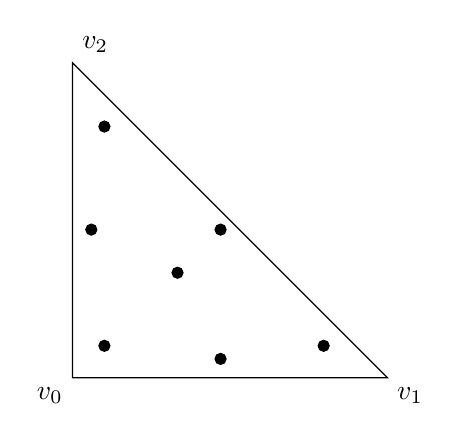
\begin{tikzpicture}[scale = 4,
]
	\def \xOneRef {0};
	\def \yOneRef {0};
	\def \xTwoRef {1};
	\def \yTwoRef {0};
	\def \xThreeRef {0};
	\def \yThreeRef {1};

	\coordinate (POneRef) at (\xOneRef, \yOneRef);
	\coordinate (PTwoRef) at (\xTwoRef, \yTwoRef);
	\coordinate (PThreeRef) at (\xThreeRef, \yThreeRef);


	\draw (0,0) -- (0,1) -- (1,0) -- cycle;

%draw point in ref triangle
	\draw[fill] (POneRef) circle (0.0pt) node [below left] {$v_0$};
	\draw[fill] (PTwoRef) circle (0.0pt)node [below right] {$v_1$};
	\draw[fill] (PThreeRef) circle (0.0pt)node [above right] {$v_2$};

	\def \a {0.470142};
	\def \b {0.0597159};
	\def \c {0.101287};
	\def \d {0.797427};
  	\draw[fill] \baryc {0.333333} {0.33333} {0.33333} circle (0.5pt);
  	\draw[fill] \baryc {\b} {\a} {\a} circle (0.5pt);
  	\draw[fill] \baryc {\a} {\b} {\a} circle (0.5pt);
 	\draw[fill] \baryc {\a} {\a} {\b} circle (0.5pt);
  	\draw[fill] \baryc {\d} {\c} {\c} circle (0.5pt);
  	\draw[fill] \baryc {\c} {\d} {\c} circle (0.5pt);
  	\draw[fill] \baryc {\c} {\c} {\d} circle (0.5pt);
\end{tikzpicture}
	\caption{Quadrature points for a integral over a triangle domain with $N=7$}
	 \label{fig: quadrature}
\end{figure}
Quadrature formulas, i.e. quadrature points and weights, especially for handling volume integrals can be found in \cite{Strout1971}.
To assemble the stiffness matrix $M$ the data we have to provide reduces to the data at the element, face respectively quadrature points.  
At an element quadrature point these are the gradients, whereas at a face quadrature point we need information about  the function values $u$ and the normal derivatives, i.e. $\nabla u \cdot \mathbf{n}$ of all test functions.

\subsection{A Reference Cell}
To reduce the storage space one usually specifies a reference cell $T_{ref}$ such that every triangle $T \in \triang$ is the image of $T_{ref}$ under an affine transformation $\Phi_T:T_{ref} \rightarrow T$. 
%We make use of the triangle spanned by the points $(0,0)^t, (0,1)^t$ and $(1,0)^t$ for our reference cell. 
Since the DG spaces also allow discontinuous functions a basis $p^1_{ref},\dots,p^n_{ref}$ of $T_{ref}$ also induces a basis on every $T$, namely the basis consisting of 
\[
	p_T^i(x) := p^i_{ref}(\Phi_T^{-1}(x)), \qquad x \in T, 1 \leq i \leq n.
\]
The most famous basis polynomials are the Lagrange elements, i.e. given a set of points $P$ each Lagrange basis element evaluate at exactly one point of $P$ to one and vanishes at every other point. Due to this property this basis is also referred as a nodal basis. 
A huge benefit of the Lagrange elements are their interpolation properties. 

Now most of the required data on a triangle $T$ can be easily derived knowing $\Phi_T$ and the reference cell $T_{ref}$. We explain how to do that in detail for the two-dimensional case.

\begin{example}\label{ex: base cell trafo}
From now an we consider $\Omega \subset \R^2$ and we choose the reference triangle to be the triangle spanned by the points $\point 0 0, \point 0 1$ and $\point 1 0$.
Suppose we want to figure out the transformation for the triangle $T = \langle v_1,v_2,v_3 \rangle$.
It has to hold
\[
\Phi\left(\point 0 0\right) = v_0, \Phi\left(\point 0 1\right) = v_1 \textnormal{ and } \Phi\left(\point 1 0\right) = v_2
\]
Since every two-dimensional affine transformation can be written in the form $\Phi(x) = Ax+b$ for some $A \in \R^{2 \times 2}$ and $b \in \R^2$ it is easy to verify that we have $A = \begin{pmatrix} v_1-v_0 & v_2-v_0\end{pmatrix}$ and $b = v_0$.
Having determined the transformation we are able to easily calculate its inverse $\Phi_T^{-1}(x) = A^{-1} (x-b) =: A^{-1} x- \tilde b$. \\
Let $\beta_0, \beta_1$ and $\beta_2$ be the barycentric coordinates of $x \in T$. Because of $\Phi^{-1}$'s linearity we find
\begin{align*}
	p^i_T(x) =& p_T^i( \beta_0 v_0 +\beta_1 v_1 + \beta_2 v_2  ) \\
	=& p^i_{ref}(\Phi_T^{-1}(\beta_0 v_0 +\beta_1 v_1 + \beta_2 v_2)) \\
	=& p^i_{ref}(\beta_0 \Phi_T^{-1}(v_0) +\beta_1 \Phi_T^{-1}(v_1) + \beta_2 \Phi_T^{-1}(v_2)) \\
		=& p^i_{ref}(\beta_0 \point 0 0 +\beta_1 \point 0 1 + \beta_2 \point 1 0 ), \qquad 1 \leq i \leq n.
\end{align*}
Thus, basis function values in $T$ can be simply determined by barycentric coordinates. Henceforth we refer with $x_{ref}$  to the point $\beta_0 \point 0 0 +\beta_1 \point 0 1 + \beta_2 \point 1 0$ which is the to $x$ corresponding point in the reference triangle . In Figure \ref{fig: transformation} the connection between $x_{ref}$ and $x$ is shown.

\begin{figure}[!h]
	
\usetikzlibrary{calc}
\usetikzlibrary{decorations.markings}
%\newcommand\fOne[2]{2*#1 + 0* #2 + 2}

%\fOne 1 1 

\begin{tikzpicture}[scale = 4,
]
	\def \xOneRef {0};
	\def \yOneRef {0};
	\def \xTwoRef {1};
	\def \yTwoRef {0};
	\def \xThreeRef {0};
	\def \yThreeRef {1};

	\coordinate (POneRef) at (\xOneRef, \yOneRef);
	\coordinate (PTwoRef) at (\xTwoRef, \yTwoRef);
	\coordinate (PThreeRef) at (\xThreeRef, \yThreeRef);

	\def \xRef {0.6};
	\def \yRef {0.2};
	\coordinate (PRef) at (\xRef, \yRef);


	\def \a {1.1};
	\def \b {0.4};
	\def \c {1.2};
	\def \d {0.3};

	\def \e {1.5};
	\def \f {0.5};

	\coordinate (xOneT) at ($({\a*\xOneRef+\b*\yOneRef+\e},{\c*\yOneRef+\d*\xOneRef+\f})$);
	\coordinate (xTwoT) at ($({\a*\xTwoRef+\b*\yTwoRef+\e},{\c*\yTwoRef+\d*\xTwoRef+\f})$);
	\coordinate (xThreeT) at ($({\a*\xThreeRef+\b*\yThreeRef+\e},{\c*\yThreeRef+\d*\xThreeRef+\f})$);

	\coordinate (xT) at ($({\a*\xRef+\b*\yRef+\e},{\c*\yRef+\d*\xRef+\f})$);


	\draw (0,0) -- (0,1) -- (1,0) -- cycle;
	\draw (xOneT) -- (xTwoT) -- (xThreeT) -- cycle;

%draw point in ref triangle
	\draw[fill] (POneRef) circle (0.6pt) node [below left] {$v^{ref}_0$};
	\draw[fill] (PTwoRef) circle (0.6pt)node [below right] {$v^{ref}_1$};
	\draw[fill] (PThreeRef) circle (0.6pt)node [above right] {$v^{ref}_2$};

	\draw[fill] (PRef) circle (0.6pt) node [left] {$x^{ref}$};


	\draw[fill] (xOneT) circle (0.6pt) node [left=0.1cm] {$v_0$};
	\draw[fill] (xTwoT) circle (0.6pt) node [right=0.2cm] {$v_1$};
	\draw[fill] (xThreeT) circle (0.6pt) node [above right] {$v_2$};

	\draw[fill] (xT) circle (0.6pt) node [left=0.1cm] {$\Phi(x^{ref}) =x$};

%	\draw[->, shorten >=0.5cm, shorten <=1cm] (PRef) edge [bend right] ($(xT)$);

	\draw[
			decoration = {markings, mark=at position 0.98 with {\arrow[scale=3, black]{stealth}}},
			postaction = {decorate},
			shorten >=5,
			shorten <=5,
			bend right] (PRef) to node [below] {{\Large $\Phi$}} ($(xT)-(0.005,0.005)$) ;

	%draw axes
	\draw[thick,->] (0, 0) -- (1.3,0);
	\draw[thick,->] (0, 0) -- (0,1.3);
	


\end{tikzpicture}
	\caption{Transformation of reference cell}
	 \label{fig: transformation}
\end{figure}

Similarly we can affiliate the determination of the gradient in $T$ to a calculation in $T_{ref}$. With the chain rule we have
\begin{align*}
	\left(\nabla_x p_T^i(x)\right)^t = D_x p_T^i(x) =& D_x p^i_{ref}(\Phi_T^{-1}(x)) \\
	  =& D_{\Phi_T^{-1}(x)}p^i_{ref}(\Phi_T^{-1}(x)) \cdot D_x  \Phi_T^{-1}(x) \\
	  =& D_{x_{ref}}p^i_{ref}(x_{ref}) \cdot  A^{-1}
\end{align*}
and thus
\begin{align}
	\nabla_x p_T^i(x) = A^{-t} \cdot \nabla_{x_{ref}}(x_{ref}), \qquad 1 \leq i \leq n. \label{eq: ref gradient}
\end{align}

Analogous proceeding yields for the Hessian matrix
\begin{align}
D_x^2p_T^i(x) = A^{-t} D_{x_{ref}}^2p^i_{ref}(x_{ref})  A^{-1}, \qquad 1 \leq i \leq n.
\end{align}

Concluding, if we need to determine function values, gradient and Hessian of a basis function on a cell, we only need the Jacobian of its transformation, i.e. $A$. We are able to calculate all further information with the data provided by the reference triangle.
\end{example}

\subsection{Refinement and Base Cells}\label{subsec: refinement and base cells}
Let us in the rest of this section further assume we have a triangulation of a two-dimensional domain $\Omega$. 
Suppose the mesh of our triangulation is created by refinement of a coarser mesh. We use a specific kind of refinement: Given a triangulation $\triang$ every triangle $T \in \triang$ is divided into four congruent triangles as is shown in figure \ref{pic: refinement}. We note, the finer grid $\triangFine$ for the diameter of each triangle is halved.

\begin{figure}[h]
\usetikzlibrary{calc}

		\begin{center}
		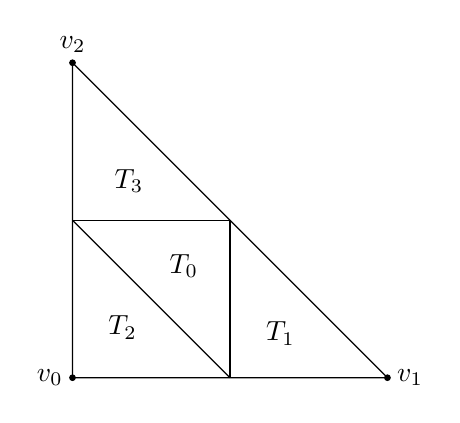
\begin{tikzpicture}
%define coordinates
			\coordinate (vEins) at (0,0) ;
			\coordinate (vZwei) at (0:4cm);
			\coordinate (vDrei) at (90:4cm);

%draw triangle
			\draw (vEins) -- (vZwei) -- (vDrei) -- cycle;

%draw refined triangle
			\draw ($(vEins)!0.5!(vZwei)$) -- ($(vEins)!0.5!(vDrei)$);
			\draw ($(vDrei)!0.5!(vZwei)$) -- ($(vEins)!0.5!(vDrei)$);
			\draw ($(vEins)!0.5!(vZwei)$) -- ($(vZwei)!0.5!(vDrei)$);

%draw nodes
			\draw[fill =black] (vEins) circle (1pt) node[left] {$ v_0$};
			\draw[fill =black] (vZwei) circle (1pt) node[right] {$v_1$};
			\draw[fill =black] (vDrei) circle (1pt) node[above] {$v_2$};

%			\draw node at (30:2.4cm) {$T_1$};

			\draw node at (45:0.9cm) {$T_2$};
			\draw node at (45:2cm) {$T_0$};
			\draw node at (74:2.6cm) {$T_3$};
			\draw node at (12:2.7cm) {$T_1$};

		\end{tikzpicture}
		\end{center}

\caption{Refinement of a triangle}
 \label{pic: refinement}
\end{figure}

We identify the new refined triangles with their original cell in $T$ calling it their basecell $T^T_b$. Repeating the refinement we can always relate a cell in the finest mesh with a basecell in the original triangulation. We can find an affine mapping $\Psi_T:T^T_b \rightarrow T$ transforming the $T^T_b$ to $T$ such that $\Phi_T = \Psi_T \circ \Phi_B$. This implies also that for the jacobians $A_{\Phi_T}, A_{\Psi_T}, A_{\Phi_B}$ of the affine transformations $\Phi_T, \Psi_T,\Phi_B$ holds
\begin{align}
A_{\Phi_T}=A_{\Psi_T} A_{\Phi_B}
\end{align} 

This makes saving information about the basecell very beneficial for the transformation matrix $A_{\Psi_T}$ is a diagonal matrix which even has the same entries along the diagonal. It even follows basis function data on two triangles with the same basecell only differ in a constant. Yet another benefit of the relation between cells and their basecells is they hav the same, or for the innermost triangle($T_0$ in figure \ref{pic: refinement}) opposite directed, normals.

\begin{example}\label{ex: leaf cell trafo}
In the two-dimensional case the Jacobian $A_{\Psi_T}$ of a transformation $\Psi_T$ from the base cell $B$ to a $l$ times refined triangle $T$ is $
	\begin{pmatrix}
		\frac 1 {2^l} & 0 \\ 0 & \frac 1 {2^l}
	\end{pmatrix} \text{ or }
	\begin{pmatrix}
		-\frac 1 {2^l} & 0 \\ 0 & -\frac 1 {2^l}
	\end{pmatrix}$, respectively if the number of intermediate basecells being an inner triangle during refinement  has been odd.

 To a point $x \in T$ we can determine a corresponding base cell point $x_B$, namely the point which satisfies $x = \Psi_T(x_B)$. With the help of \eqref{eq: ref gradient} we find the identity
\begin{align}
\nabla_x p_T^i(x) &= A_{\Phi_T}^{-t} \nabla_{x_{ref}} p^i_{ref} (x_{ref}) \nonumber\\
 &= A_{\Psi_T}^{-t} A_{\Phi_B}^{-t} \nabla_{x_{ref}} p^i_{ref} (x_{ref}) \nonumber\\
&= \epsilon 2^l A_{\Phi_B}^{-t} \nabla_{x_{ref}} p^i_{ref}(x_{ref}), \qquad \epsilon \in \{+,-\} \label{eq: trafo grad},
\end{align}
with $l \in \N$ indicating how often $T$ is refined with respect to the original mesh.\\
Analogously we have
\begin{align}
\nabla_x p^i(x) \mathbf n &= 2^l  A_{\Phi_B}^{-t} \cdot \nabla_{ref}p^i_{ref}(x_{ref}) \mathbf{ n_{b}} \qquad \text{ and } \label{eq: trafo normal der} \\
D_x^2 p^i(x) &= 2^{2l}  A_{\Phi_B}^{-t} D_{x_{ref}}^2 p^i_{ref}(x_{ref}), \qquad 1 \leq i \leq n,
\end{align}
where $\mathbf n_b$ is the to $n$ corresponding normal in the base cell. Note, that \eqref{eq: trafo normal der} even holds for inner refined triangles: The minus sign of the gradient cancels with the minus sign of the base cell normal $n_B$ since $n_B$ is opposite directed as the corresponding normal $n$ of a inner triangle.\\
Another case where the sign of the gradient \eqref{eq: trafo grad} could be important when we evaluate of the first part of the bilinearform, i.e. $\nabla \phi \cdot A \nabla v$. We first note, that two basis functions $p_T^i, p_T^j$ having only support on $T$ are created with the same affine mapping $\Phi_T$. Hence they have the same transposed, inversed Jacobian $A^{-t}_{\Phi_T}=\epsilon 2^l A_{\Phi_b}^{-t}$ and therefore the sign on the right-hand side in \eqref{eq: trafo grad} is for both gradients the same. Because we multiply both gradients a sign change between base and the actual cell does not affect the evaluation of our bilinear form. 
Of course for other combinations of basis polynomials the latter volume integral always equals zero because the polynomials' support is chosen in such a way that all other gradients vanish in the inner of $T$.

A usual error source are the signs of the terms
\[
	\jump {\varphi \average{ A \nabla v }} = \varphi^+ \frac 1 2  \left(A^+ \nabla v^+ + A^- \nabla v^-\right) \cdot \mathbf n^+ + \varphi^- \frac 1 2 \left(A^+ \nabla v^+ + A^- \nabla v^-\right) \cdot \mathbf n^-.
\]
Since for two adjacent triangles always $\mathbf n^+ = - \mathbf n^-$ holds, we also have $A^+ \nabla v^+ \mathbf n^-= -A^+ \nabla v^+ \mathbf n^+$ and $A^- \nabla v^- \mathbf n^+= -A^- \nabla v^- \mathbf n^-$. Hence we can calculate the expression using \ref{eq: trafo normal der}. Note that all basic functions have support on only one triangle, such that for a evaluation of a basic functions $\varphi_B$ either $\varphi_B^+$ or $\varphi_B^-$, just as for a basic functions $v_B$ either $v_B^+$ or $v_B^-$ equals to zero.

So, we are able to save a lot of memory if we store instead of all data at every quadrature points in each refined cell just the data of the base cell and the number of refinements. The refined cells contained in the actual mesh are referred as \emph{leaf cells}.
\end{example}

\subsection{Assembly Loop}
Another crux of the implementation is the handling of face terms, more specific: We mentioned earlier that we evaluate the bilinearform cell-wise. Hence the volume integrals are calculated visiting every cell only once. When do we compute the edge integrals?\\
Face terms can be collected either by assemble them in two steps or a more complex one.
For the two step variant the face terms are split up into the contributions of their two adjacent cells, such that the first part is assembled when processing the first adjacent cell and the second during the processing of the other adjacent cell. \\
In the one step variant we handle a face term when visiting an adjacent cell for first time. To detect the first time we introduce a cell flag for every leaf cell indicating whether the cell has been processed yet. Now, each time the assembling algorithm visits a face it determines the neighbouring cell and checks if the face has already been processed. The following algorithm \ref{alg: assembling} from \cite{BMV2009} illustrates how to perform this one step approach. 
\begin{algorithm}[H]
\caption{An assembling loop for a DG method}
\label{alg: assembling}
\begin{algorithmic}
\Ensure every cell flag is false
\For {cell in all leaf cells}  
\State get cell data
\State assemble volume integrals 
	\For {face in faces(cell)}
		\If {neighbour across the face exists} 
			\If {not neighbour flag}
					\State get neighbour cell data
					\State assemble face terms
			\EndIf
		\Else
			\State assemble boundary terms
		\EndIf
\EndFor
	\State cell flag to true 
\EndFor
\State Reset every cell flag to false
\end{algorithmic}
\end{algorithm}

In \cite{BMV2009} Brix et. alter also develop a data structure efficiently handling all the mentioned requirements among a lot of other features. On this structure our implementation used for the later numerical results is based on.

After we saw the main implementation points of a DG method we need some algebraic and analytic identities for the Hessian matrix to develop a DG method handling the \MA equation.
\section{Hessian Identities}

We begin with the notion of the cofactor matrix which is later important for the linearisation of the \MA equation.
\begin{definition}[Cofactor Matrix] \label{def: cof matrix}
	The \emph{cofactor matrix} of a matrix $A \in \R^{d \times d}$ is defined by the entries
	\begin{align}
	(\mycof A )_{i,j} = (-1)^{i+j} \mydet{A_{ij}},
	\end{align}
	where $A_{ij}$ denotes the matrix resulting from deleting the $i$-th row and $j$-column in $A$.
\end{definition}

We observe that in the two-dimensional case the cofactor matrix of the Hessian simplifies to
\begin{align}
\mycof {D^2 u} = \begin{pmatrix}
								\dxx{x_2} u & -\frac {\partial }{\partial x_1 x_2} u\\
								-\frac {\partial }{\partial x_2 x_1} u & \dxx{x_1} u
							\end{pmatrix}.
\end{align}

\begin{definition}[Frobenius product]
	The Frobenius product : of two matrices $A, B \in R^{d \times d}$ is defined by
	\[
		A:B := \sum_{1 = i,j} ^d a_{i,j} b_{i,j}
	\]
\end{definition}

Very helpful is the relation between the determinant and the cofactor matrix.
\begin{lemma}\label{la: rel det cofactor}
	For every matrix $A  \in \R^{d \times d}$ it holds
	\[
		d \mydet A = \mycof A: A
	\]
\end{lemma}
\begin{proof}
	After Laplace's formula it holds for any $1 \leq j \leq d$
	\[
		\mydet A = \sum\limits_{i = 1}^{d} a_{i,j} (\mycof A )_{i,j} 
	\]
	Summing over all $j$ yields
	\[
		d \mydet A = \sum\limits_{j= 1}^{d} \sum\limits_{i = 1}^{d} (\mycof A )_{i,j}  a_{i,j}  = \mycof A: A
	\]
\end{proof}

Another advantage is the behaviour of the cofactor matrix of a Hessian if a divergence is applied to it:
\begin{definition}[Matrix Divergence]
The divergence $\nabla \cdot A$ for a matrix $A$ is defined by taking the divergence row-wise,i.e.
\[
	\nabla \cdot A := \begin{pmatrix} \nabla \cdot A_1 \\ \vdots \\ \nabla \cdot A_d\end{pmatrix}
	= \begin{pmatrix} \sum_{j = 1}^{d} \dx{x_i} a_{1,j} \\ \vdots \\ \sum_{j = 1}^{d} \dx{x_i} a_{d,j}\end{pmatrix}.
\]
where $A_i$ denotes the $i$-th row of $A$.
	
\end{definition}

\begin{lemma}[Divergence-Free Property of Cofactor Matrices] \label{la: divergence free cof}
For smooth functions $u:\Omega \rightarrow \R$ with $\Omega \subset \R^2$ the cofactor matrix of the Hessian is divergence-free:
\[
	\nabla \cdot \mycof{D^2 u} = 0.
\] 
\end{lemma}
\begin{proof}
\begin{align*}
	\nabla \cdot \mycof{D^2 u} = \sum_{i=1}^{d} \dx{ x_i}\mycof{D^2 u}_i = 
	\begin{pmatrix}
		\frac {\partial^3} {\partial x_1 {x_2}^2 } -\frac {\partial^3} {\partial{x_2} x_1 {x_2}} \\
				\frac {\partial^3} {\partial {x_1}x_2 {x_1}} -\frac {\partial^3} {\partial x_2 {x_1}^2 }
	\end{pmatrix}
\end{align*}
By Schwarz' theorem the latter equals zero if $u$ is twice continuous differentiable.
\end{proof}

The divergence-free property yields to a integration by parts rule:
\begin{lemma}[Integration by parts for the Frobenius product] \label{la: integration by parts Frobenius}
For a Frobenius product with the Hessian's cofactor matrix  the following integration by parts rule holds for smooth $u$
\[
	\int_\Omega (D^2 u : B) = - \int_\Omega (\nabla \cdot B) \cdot \nabla u + \int_{\partial \Omega}  B \nabla u \bf n
\] 
\end{lemma}

\begin{proof}
The proof is based on applying integration by parts row-wise
\begin{align*}
- \int_\Omega (\nabla \cdot B) \cdot \nabla u &= 
- \int_\Omega \sum_{i = 1}^{d} (\nabla \cdot B_i) \dx {x_i} u \\
&=  \int_\Omega \sum_{i = 1}^{d} B_i \cdot  (\nabla \dx {x_i} u) - \int_{\partial \Omega} \sum_{i = 1}^{d} (B_i) \dx {x_i} u \mathbf{n} \\
&=  \int_\Omega \sum_{i = 1}^{d}\sum_{j= 1}^{d} B_{ij} \dxy {x_i}{x_j} u- \int_{\partial \Omega} B \nabla u \mathbf{n} \\
&=  \int_\Omega (D^2 u : B)- \int_{\partial \Omega} B \nabla u \mathbf{n} 
\end{align*}
\end{proof}

When later talking about weak formulations it is handy to have a divergence form of the latter Frobenius product.
\begin{lemma}[Divergence form of the Frobenius Product] \label{la: An application of the divergernce product rule}
\[
		\nabla \cdot \left( \mycof {D^2 u } \nabla v \right) %- \nabla \cdot \left(\mycof {D^2 u }\right) \nabla v
		= \mycof {D^2 u}: D^2 v
\] 
\end{lemma}

\begin{proof}
\begin{align*}
\nabla \cdot \left( \mycof {D^2 u } \nabla v \right) =&%- \nabla \cdot \left(\mycof {D^2 u }\right) \nabla =& 
\sum_{i= 1}^{d} \dx {x_i} 	\left( \sum_{j= 1}^{d} \mycof {D^2 u }_{i,j} \dx{x_j} v \right)\\
%&-  \sum_{j= 1}^{d}  \sum_{i= 1}^{d} \left(\dx {x_i} \mycof {D^2 u }_{i,j}  \right) \dx{x_j} v \\
=&  \sum_{i= 1}^{d} \sum_{j= 1}^{d}  \left(\dx {x_i} \mycof {D^2 u }_{i,j}  \right) \dx{x_j}v + \sum_{i= 1}^{d} \sum_{j= 1}^{d}  \mycof {D^2 u }_{i,j} \dxy{x_j}{x_i}v\\
=&  \sum_{j= 1}^{d}  \nabla \cdot \left(\mycof {D^2 u }\right)_j \dx{x_j}v + \sum_{i= 1}^{d} \sum_{j= 1}^{d}  \mycof {D^2 u }_{i,j} \dxy{x_j}{x_i}v\\
=&   \nabla \cdot \left(\mycof {D^2 u }\right) \nabla v+ \mycof {D^2 u }:D^2v
\end{align*}
The statement results from the fact that the cofactor matrix of the Hessian is divergence-free.
\end{proof}
